\documentclass[UTF-8,fontset = none]{ctexbeamer}

\usepackage{ctex, hyperref}
\usepackage[T1]{fontenc}
\usepackage{xeCJK}

%中文字体设置为华文细黑,英文字体设置为Times New Roman
\setCJKsansfont{STXihei}
\setsansfont{Times New Roman}

% other packages
\usepackage{latexsym,amsmath,multicol,xcolor,booktabs,calligra,subfigure}
\usepackage{graphicx,pstricks,listings,stackengine,bm}
\usepackage{SYSU}

\author{孙悟空}
\title{Model of SYSU Beamer}
\subtitle{中山大学Beamer模板}
\institute{中山大学计算机学院}
\date{\today}

% defs
\def\cmd#1{\texttt{\color{red}\footnotesize $\backslash$#1}}
\def\env#1{\texttt{\color{blue}\footnotesize #1}}
\definecolor{deepblue}{rgb}{0,0,0.5}
\definecolor{deepred}{RGB}{116,0,3}
\definecolor{deepgreen}{RGB}{0,88,37} %中大专属绿色

\lstset{
    basicstyle=\ttfamily\small,
    keywordstyle=\bfseries\color{deepblue},
    emphstyle=\ttfamily\color{deepred},    % Custom highlighting style
    stringstyle=\color{deepgreen},
    numbers=left,
    numberstyle=\small\color{halfgray},
    rulesepcolor=\color{red!20!green!20!blue!20},
    frame=shadowbox,
}

\begin{document}

\begin{frame}
    \titlepage
    \begin{figure}[htpb]
        \begin{center}
            \subfigure{
\includegraphics[width=0.1\linewidth]{pic/SYSULogo.jpg}}
            \subfigure{
\includegraphics[width=0.1\linewidth]{pic/CSELogo.jpg}}
        \end{center}
    \end{figure}
\end{frame}

\begin{frame}
    \tableofcontents[sectionstyle=show,subsectionstyle=show/shaded/hide,subsubsectionstyle=show/shaded/hide]
\end{frame}


\section{基本环境配置}

\begin{frame}{itemize应用案例}
    \begin{itemize}
    \item \bfseries{什么是自监督学习?} 
        \begin{itemize} 
            \item 利用辅助任务(Pretext)从大规模无监督数据中挖掘监督信息
            \item 利用Pretext构造的监督信息对网络进行训练,学习有价值的Semantic Representation
            \item 针对不同的下游任务,利用Fine Tuning完成预训练模型的适配
        \end{itemize}
    \item \bfseries{什么场景需要自监督学习?}
        \begin{itemize}
            \item 制作有完整标签的数据集需要耗费大量成本。
            \item 对数据集本身的语义特征进行提取。
        \end{itemize}
    \item \bfseries{自监督学习常用的方法有哪几类?}
        \begin{itemize}
            \item 基于上下文信息:拼图、抠图、颜色预测、旋转等
            \item 基于时序:帧的相对位置、同一帧多视角、追踪框等
            \item 基于对比:基于正样本、负样本、锚(anchor)点相似性度量
        \end{itemize}
    \end{itemize}
\end{frame}

\begin{frame}{三线表应用案例}
    \begin{table}[htpb]
        \centering
        \label{tab:BERTModel}
        \begin{tabular}{lll}
            \toprule
            模型参数 & $BERT_{base}$ & $BERT_{large}$ \\ 
            \midrule
            Transformer层数L & 12 & 24 \\
            Hidden Units(H) & 768 & 1024 \\
            Self-attention Heads(A) & 12 & 16 \\
            参数总量 & 110M & 340M\\ 
            \bottomrule
        \end{tabular}
    \end{table}
    文中有两个模型,一个是base模型,一个是large模型,设计两个模型主要是为了研究数据量与模型规模对训练效果的影响。
\end{frame}

\begin{frame}{有色表格应用案例}
    \begin{table}[htbp]
        \centering
        \begin{tabular}{c|c}
        \hline
        $f(x)$           & $f^{\prime}(x)$    \\ \hline
        $x^k$            &  $kx^{k-1}$        \\
        $e^x$            & $e^x$              \\
        $a^x(a>0)$       & $a^{x}\ln(a)$      \\
        $\ln(x)$         & $1/x$              \\
        $\log_{a}(x)(a>0,a\neq 1)$   & $1/x\ln(a)$  \\                                                                                      
        $\sin(x)$        & $\cos(x)$          \\
        $\cos(x)$        & $-\sin(x)$         \\
        $\arcsin(x)$     & $1/\sqrt{1-x^2}$   \\
        $\arccos(x)$     & $-1/\sqrt{1-x^2}$  \\ \hline
        \end{tabular}
        \label{tab:deriva}
    \end{table}
    上表详细介绍了各个基本初等函数的导数。
\end{frame}

\section{Case1 原模型BERT}

\subsection{模型结构与表征提取}

\begin{frame}{block环境的应用}
    \begin{alertblock}{相对误差估计分析}
        $\frac{\|\delta x\|}{\|x\|}<\frac{\|\bm{A}^{-1}\|\cdot\|\delta\bm{A}\|}{1-\|\bm{A}^{-1}\|\cdot\|\delta\bm{A}\|}$     
    \end{alertblock}
    \begin{block}{重要函数:误差函数}
       \begin{equation*}
           erf(x) = \frac{2}{\sqrt{\pi}}\int_{0}^{x}e^{-t^2}dt 
           \label{eq:erfF}
       \end{equation*}
    \end{block}
\end{frame}

\subsection{模型训练过程分析}
\begin{frame}{Pre-training\& Fine-Tuning}
    \begin{figure}[htpb]
        \begin{center}
            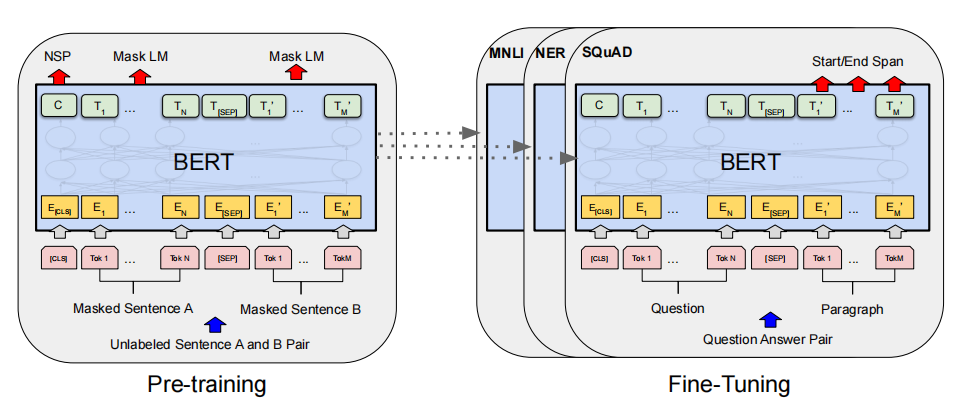
\includegraphics[width = 1\linewidth]{pic/StepOfBERT.png}
        \end{center}
    \end{figure}
\end{frame}

\begin{frame}{步骤分析}
\begin{itemize}
    \item \bfseries{Pre-training} 
    \begin{itemize} 
        \item MLM(Masked Language Model) $\rightarrow$ Context based
        \item NSP(Next Sentence Prediction) $\rightarrow$ Temporal based
    \end{itemize}
    \item \bfseries{Fine-Tuning} \\
    Transformer的自注意力机制使得BERT在替换少量的输入与输出后可以直接用于每个下游任务的建模: 
    MNLI, QQP, SST-2, CoLA, SQuAD \dots
\end{itemize}
\end{frame}

\section{Case2 草图格式塔模型Sketch BERT}

\subsection{模型训练过程}

\begin{frame}{Embedding构建}
    \begin{block}{三类Embeddinng}
        与BERT类似,作者构建了三类Embedding:
        \begin{equation*}
            \begin{cases}
             E_{pt} = W_{pt}(\Delta x,\Delta y,p_{1},p_{2},p_{3})^{T}\\
             E_{ps} = W_{ps}l_{ps} \in R^{d_{E}}\\
             E_{str} = W_{str}l_{str} \in R^{d_{E}}\\
             E=E_{pt}+E_{ps}+E_{str}
            \end{cases} 
            \label{eq:1}
        \end{equation*}
    \end{block}
\end{frame}

\begin{frame}{自监督学习模型SGM}
    \begin{itemize}
        \item \textbf{位置信息的掩膜。} 划分笔划内点的偏移与笔划起始点的偏移,等比例采样\cite{2020Sketch}
        \item \textbf{状态信息的掩膜。} 基于$p_{1}, p_{2}, p_{3}$的数量等比例采样,设置$p_{1}=p_{2}=p_{3}=0$
        \item \textbf{Embedding重构网络。} SGM引入了一个Embedding重构网络,作为Refine Embedding网络相应的解码器
    \end{itemize}
\end{frame}

\subsection{下游任务评估}
\begin{frame}{下游任务List}
    \begin{figure}[htpb]
        \begin{center}
            \subfigure{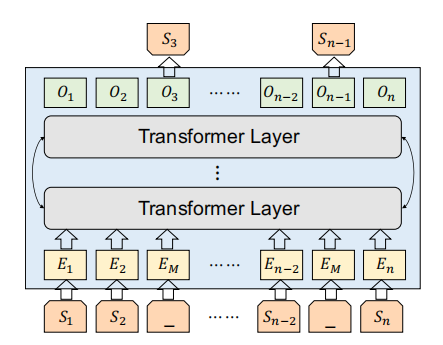
\includegraphics[width=0.3\linewidth]{pic/SkBERT-A.png}}
            \subfigure{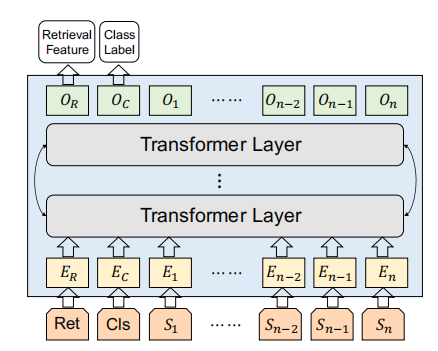
\includegraphics[width=0.3\linewidth]{pic/SkBERT-B.png}}
        \end{center}
    \end{figure}
    \begin{itemize}[<+-| alert@+>] % 当然,除了alert,手动在里面插 \pause 也行
        \item \textbf{草图识别}——添加[CLS]Token,Softmax分类,交叉熵损失
        \item \textbf{草图检索}——添加[RET]Label,交叉熵损失
        \item \textbf{草图格式塔}——直接应用SGM进行分类
    \end{itemize}
\end{frame}

\section{总结与疑问}

\subsection{两个模型的对比与总结}
\begin{frame}
    针对两个模型的对比如下:
    \begin{table}[h]
        \centering
        \begin{tabular}{c|cc}
            模型 & BERT & SketchBERT \\ \hline
            场景 & 自然语言预测 & 草图补全 \\
            Data & 单语种语料库 & QuickDraw\&TU-Berlin \\
            Pretext & MLM\&NSP & SGM \\
            Embedding & T,S,P & pt,ps,str\\
            Downstream & GLUE & 识别/检索/Gestalt \\
        \end{tabular}
    \end{table}
\end{frame}

\subsection{个人的疑问}
\begin{frame}
    \begin{itemize}
        \item 问题一:如果能学习到笔划顺序重要性的语义特征,Sketch自监督学习能力能否有所提升?
        \item 问题二:Sketch-BERT中的Embedding Matrix是怎么训练得到的?       
        \item 问题三:Fine-Tuning: Trick or Transfer Learning Theory?
    \end{itemize}
\end{frame}

\section{参考文献}

\begin{frame}[allowframebreaks]
    \bibliography{ref}
    \bibliographystyle{alpha}
    % 如果参考文献太多的话,可以像下面这样调整字体:
    % \tiny\bibliographystyle{alpha}
\end{frame}

\begin{frame}
    \begin{center}
        {\Huge\calligra Thanks!}
    \end{center}
\end{frame}

\end{document}
